\appendix
\section{Detailed estimator derivations}
\label{app:theory}

The main text gives the estimator, its unbiasedness identity, and the unified
variance analysis. This appendix supplies the detailed Top-$k$ bias
derivations and the single-control oracle calculation, including the
boundary-term cancellation for the complete coarse distribution.

\subsection{Three biased forms of Teacher \texorpdfstring{Top-$k$}{Top-k} reverse KL}
\label{app:topk-bias}

This subsection distinguishes three operations that are often conflated:
renormalizing both distributions on the head, truncating the scalar reverse-KL objective, and truncating only the stopped-coefficient gradient. Each is
computable from Teacher Top-$k$, but none generally estimates correctly the gradient of full-vocabulary reverse KL. Here ``bias'' is relative to that target gradient, not Monte Carlo sampling bias. Fix the support $S$ and Teacher probabilities,
let $z$ be unrestricted Student logits, and define
\begin{equation}
 \begin{gathered}
 R\coloneqq\sum_i p_i r_i=\KL(p\|q),\qquad
 R_S\coloneqq\sum_{i\in S}p_i r_i,\\
 P\coloneqq\sum_{i\in S}p_i,\qquad
 Q\coloneqq\sum_{i\in S}q_i.
 \end{gathered}
\end{equation}
The exact full-rKL logit gradient, which provides the reference below, is
\begin{equation}
 [\nabla_z R]_j=p_j(r_j-R).
 \label{eq:full-rkl-logit-gradient}
\end{equation}

\paragraph{Renormalized Top-$k$ reverse KL.}
Define $\widetilde p_i=p_i/P$, $\widetilde q_i=q_i/Q$ and
$\widetilde r_i=\log(\widetilde p_i/\widetilde q_i)$ for $i\in S$, with
$\widetilde R=\sum_{i\in S}\widetilde p_i\widetilde r_i$. Since
$\widetilde p_i=\exp (z_i)/\sum_{\ell\in S}\exp (z_\ell)$, the objective and its
logit gradient are
\begin{equation}
 \begin{aligned}
 L_{\mathrm{renormalized}}
 &=\sum_{i\in S}\widetilde p_i
   \log\frac{\widetilde p_i}{\widetilde q_i},\\
 [\nabla_z L_{\mathrm{renormalized}}]_j
 &=\ind\{j\in S\}\widetilde p_j
   (\widetilde r_j-\widetilde R).
 \end{aligned}
 \label{eq:renorm-topk-gradient}
\end{equation}
Every tail-logit component is exactly zero, whereas
Equation~(\ref{eq:full-rkl-logit-gradient}) is generally nonzero there. The
global minimum is the set
\begin{equation}
 \widetilde p_i=\widetilde q_i
 \quad(i\in S)
 \quad\Longleftrightarrow\quad
 p_i=\frac{P}{Q}q_i\quad(i\in S),
 \label{eq:renorm-topk-optimum}
\end{equation}
with arbitrary $P$ and arbitrary tail shape. Renormalization therefore learns
only the conditional head distribution; it identifies neither head mass nor
the omitted conditional distribution.

\paragraph{Scalar-truncated Top-$k$ reverse KL.}
The unnormalized scalar shortcut is
$L_{\mathrm{truncated}}=R_S=\sum_{i\in S}p_i r_i$. Writing
$C_S\coloneqq\sum_{i\in S}p_i(r_i+1)=R_S+P$, direct differentiation gives
\begin{equation}
 \begin{aligned}
 \nabla_\theta L_{\mathrm{truncated}}
 &=\bhead+\nabla_\theta P,\\
 [\nabla_z L_{\mathrm{truncated}}]_j
 &=\ind\{j\in S\}p_j(r_j+1)-p_jC_S.
 \end{aligned}
 \label{eq:scalar-truncated-gradient}
\end{equation}
Thus its bias relative to full rKL is
$\nabla_\theta P-\tau_p\bmean_{\mathrm{tail}}$. In particular, for
$j\notin S$, $[\nabla_z L_{\mathrm{tr}}]_j=-p_jC_S$; when $C_S>0$,
gradient descent increases every omitted logit.

The corresponding global optimum makes the failure more explicit. For each
head coordinate,
\begin{equation}
 x\log\frac{x}{q_i}\geq-\frac{q_i}{e},
 \qquad\text{with equality iff }x=\frac{q_i}{e}.
\end{equation}
Because $\sum_{i\in S}q_i/e=Q/e<1$, all coordinatewise minima are jointly
feasible, and therefore
\begin{equation}
 p_i^\star=\frac{q_i}{e}\quad(i\in S),\qquad
 P^\star=\frac{Q}{e},\qquad
 \sum_{j\notin S}p_j^\star=1-\frac{Q}{e},
 \label{eq:scalar-truncated-optimum}
\end{equation}
with arbitrary allocation inside the tail. Even if $Q$ is near one, this
objective prefers roughly $1-1/e$ Student mass outside the Teacher head; the
tail-push is thus an objective-level property, not merely a transient gradient
sign.

\paragraph{Stopped-coefficient Top-$k$ reverse-KL gradient.}
Stopping the coefficients removes the $\nabla P$ boundary term, yet leaves the tail expectation uncorrected:
\begin{equation}
  \begin{gathered}
    \bgrad_{\text{Top-}k} \coloneqq \sum_{i \in S} \operatorname{stopgrad}(p_i r_i) \bscore_i = \bhead, \\
    [\bgrad_{\text{Top-}k}]_j = \ind\{j \in S\} p_j r_j - p_j R_S, \qquad
    \bgrad_{\text{Top-}k} - \bgrad = -\tau_p \bmean_{\mathrm{tail}}.
  \end{gathered}
  \label{eq:stopped-topk-gradient-bias}
\end{equation}
In unrestricted categorical-logit space with a non-empty tail, vanishing gradients ($\bgrad_{\text{Top-}k} = \mathbf{0}$) force $R_S = 0$ via the tail components ($j \notin S$), which subsequently implies $r_i = 0$ for all head components ($i \in S$). Consequently, $p_i = q_i$ on the head, correctly matching the aggregate tail mass ($1 - P = 1 - Q$); however, the conditional distribution over the tail remains unconstrained and arbitrary. While this stopped-gradient formulation alters the underlying target the least among the three heuristics, it remains inherently biased whenever the tail vector is non-zero. HETS and ResOPD resolve this residual bias by introducing a sampled tail correction to restore the missing expectation.

\subsection{Single-control residualization and its variance optimum}
\label{app:single-control}

Use the head/tail notation of Equation~(\ref{eq:head-tail-definitions}), let
$J=\ind\{A\notin S\}$, and let $\bm B$ be any finite prefix-measurable vector
stopped before sampling $A\sim p$. Consider the one-control estimator
\begin{equation}
 \widehat{\bgrad}(\bm B)
 \coloneqq
 \bhead+\tau_p\bm B+J(\btoken_A-\bm B).
 \label{eq:single-control-estimator}
\end{equation}
It is unbiased for every such $\bm B$:
\begin{equation}
 \E[\widehat{\bgrad}(\bm B)]
 =\bhead+\tau_p\bm B
  +\tau_p(\bmean_{\mathrm{tail}}-\bm B)
 =\bgrad.
 \label{eq:single-control-unbiased}
\end{equation}
Conditioned on $J=0$, its value is the deterministic vector
$\bhead+\tau_p\bm B$. Conditioned on $J=1$, its mean is
$\bhead+\tau_p\bm B+\bmean_{\mathrm{tail}}-\bm B$ and its covariance is
$\Cov_{\mathrm{tail}}(\btoken_A)$. The two conditional means differ by
$\bmean_{\mathrm{tail}}-\bm B$. Hence the law of total covariance gives
\begin{equation}
 \mathcal V(\widehat{\bgrad}(\bm B))
 =\tau_p\mathcal V_{\mathrm{tail}}(\btoken_A)
 +P\tau_p\lVert\bmean_{\mathrm{tail}}-\bm B\rVert_2^2.
 \label{eq:single-control-variance}
\end{equation}
The first term is independent of $\bm B$. Therefore, whenever
$0<P<1$, the unique trace-covariance minimizer and its exact regret are
\begin{equation}
 \begin{aligned}
 \bm B^\star&=\bmean_{\mathrm{tail}},\\
 \mathcal V(\widehat{\bgrad}(\bm B))
 -\mathcal V(\widehat{\bgrad}(\bmean_{\mathrm{tail}}))
 &=P\tau_p\lVert\bm B-\bmean_{\mathrm{tail}}\rVert_2^2.
 \end{aligned}
 \label{eq:single-control-oracle}
\end{equation}
The oracle removes all head-versus-tail event variance, but it is unavailable
under a sparse Teacher interface because it requires the full conditional
fine-tail mean.

HETS and ResOPD are the two payload-compatible choices
\begin{equation}
 \widehat{\bgrad}^{\mathrm{HETS}}=\widehat{\bgrad}(\bm 0),
 \qquad
 \widehat{\bgrad}^{\mathrm{ResOPD}}=\widehat{\bgrad}(\bmean_B).
\end{equation}
Their regrets relative to the single-control oracle are respectively
$P\tau_p\lVert\bmean_{\mathrm{tail}}\rVert_2^2$ and
$P\tau_p\lVert\bmean_{\mathrm{tail}}-\bmean_B\rVert_2^2$. Subtraction yields
\begin{equation}
  \mathcal{V}(\widehat{\bgrad}^{\mathrm{HETS}}) - \mathcal{V}(\widehat{\bgrad}^{\mathrm{ResOPD}}) = P\tau_p \!\left( 2\langle\bmean_{\mathrm{tail}}, \bmean_B\rangle - \lVert\bmean_B\rVert_2^2 \right).
  \label{eq:hets-cfr-variance-appendix}
\end{equation}
Thus ResOPD has lower trace covariance exactly when $\bmean_B$ is closer to
$\bmean_{\mathrm{tail}}$ than the HETS control $\bm 0$ is; no unconditional
ordering is asserted.

It remains to verify why $\bmean_B$ is available without the fine Teacher
tail. The reverse KL of the complete coarse distribution over the $k$ head
tokens and one tail bucket is
\begin{equation}
 L_{\mathrm{coarse}}
 \coloneqq
 \sum_{i\in S}p_i\log\frac{p_i}{q_i}
 +\tau_p\log\frac{\tau_p}{\tau_q}.
\end{equation}
Since
$\nabla\tau_p=\tau_p\bar{\bscore}_{\mathrm{tail}}=-\nabla P$,
direct differentiation
gives
\begin{equation}
 \begin{aligned}
 \nabla L_{\mathrm{coarse}}
 &=\bhead+\nabla P+(b+1)\nabla\tau_p\\
 &=\bhead+b\nabla\tau_p
  =\bhead+\tau_p\bmean_B
  =\bgrad_{\mathrm{coarse}}.
 \end{aligned}
\end{equation}
The boundary terms cancel because the tail pseudo-token completes the coarse
support. This is why $\bgrad_{\mathrm{coarse}}$ is an exact gradient (but biased), even though
$\bmean_B$ need not equal the true conditional fine-tail mean.

\FloatBarrier
\section{Detailed training and evaluation configurations}
\label{app:hyperparameters}


Tabs.~\ref{tab:opd-hyperparameters} and~\ref{tab:qwen3-opd-hyperparameters}
collect the complete settings for the primary mathematics and cross-domain
runs. Their sampling assumptions are discussed in
Secs.~\ref{subsec:evidence} and~\ref{sec:ex-setup}; the matched
full-support mathematics ablation is reported in
Sec.~\ref{sec:rollout-ablation}.

\begin{table}[t]
\caption{\textbf{Primary Math OPD experimental configurations and hyperparameters.}}
\label{tab:opd-hyperparameters}
\centering
\small
\renewcommand{\arraystretch}{1.18}
\setlength{\tabcolsep}{6pt}
\begin{tabular}{@{}lll@{}}
\toprule
\textbf{Category} & \textbf{Hyperparameter} & \textbf{Configuration / Value} \\
\midrule

\multirow{2}{*}{\textbf{Models}}
& Student model & Qwen3.5-4B \\
& Teacher model & Qwen3.5-27B \\
\midrule

\multirow{2}{*}{\textbf{Data}}
& Training dataset & 1{,}024 prompts sampled from DeepMath-103K \\
& Max prompt length & 2{,}048 \\
\midrule

\multirow{5}{*}{\textbf{Sampling}}
& Enable thinking & True \\
& Max response length & 32{,}768 (training and evaluation) \\
& temperature & 1.0 \\
& top-$p$ & 0.95 \\
& top-$k$ & 20 \\
\midrule

\multirow{5}{*}{\textbf{Training}}
& Training epochs & 3 \\
& Global batch size & 16 \\
& Optimizer & AdamW \\
& Gradient clipping & 1.0 \\
& Learning rate & $1\times10^{-6}$ \\
\midrule

\multirow{4}{*}{\textbf{System \& Hardware}}
& Compute infrastructure & $16\times$ NVIDIA H200 GPUs \\
& Resource allocation & 8 GPUs for Student rollout, 4 for Student training, \\
& & 4 for hosting the Teacher inference service \\
& Software frameworks & Training: verl \quad Inference: vLLM \\
\bottomrule
\end{tabular}
\end{table}

% \begin{table}[t]
% \caption{\textbf{Cross-domain Qwen3 OPD experimental configurations and hyperparameters.}}
% \label{tab:qwen3-opd-hyperparameters}
% \centering
% \small
% \renewcommand{\arraystretch}{1.18}
% \setlength{\tabcolsep}{6pt}
% \begin{tabular}{@{}lll@{}}
% \toprule
% \textbf{Category} & \textbf{Hyperparameter} & \textbf{Configuration / Value} \\
% \midrule
% \multirow{2}{*}{\textbf{Models}}
% & Student model & Qwen3-4B \\
% & Teacher model & Qwen3-30B-A3B-Instruct-2507 \\
% \midrule
% \multirow{3}{*}{\textbf{Data}}
% & Training dataset & 30,000 deduplicated prompts; \\
% & & Math/Code/Science: 10,000 each \\
% & Max prompt length & 1,024 \\
% \midrule
% \multirow{5}{*}{\textbf{Sampling}}
% & Enable thinking & False \\
% & Max response length & 8192 (training) and 32768 (evaluation) \\
% & temperature & 1.0 \\
% & top-$p$ & 1.0 \\
% & top-$k$ & $-1$ \\
% \midrule
% \multirow{7}{*}{\textbf{Training}}
% & Training steps & 100 \\
% & Global batch size & 288 \\
% & Optimizer & AdamW \\
% & Gradient clipping & 1.0 \\
% & Peak learning rate & $5\times10^{-6}$ \\
% & LR schedule & 10-step warmup; \\
% & & cosine decay to $0.1\times$ peak \\
% \midrule
% \multirow{4}{*}{\textbf{System \& Hardware}}
% & Compute infrastructure & $16\times$ NVIDIA H200 GPUs \\
% & Resource allocation & 8 GPUs for student rollout, 4 for student training, \\
% & & 4 for hosting the teacher inference service \\
% & Software frameworks & Training: verl \quad Inference: vLLM \\
% \bottomrule
% \end{tabular}
% \end{table}

\section{Step-wise evaluation results}

\subsection{Math OPD experiments}
\label{app:math-learning-trajectories}

\begin{table}[t]
\caption{\textbf{Cross-domain Qwen3 OPD experimental configurations and hyperparameters.}}
\label{tab:qwen3-opd-hyperparameters}
\centering
\small
\renewcommand{\arraystretch}{1.18}
\setlength{\tabcolsep}{6pt}
\begin{tabular}{@{}lll@{}}
\toprule
\textbf{Category} & \textbf{Hyperparameter} & \textbf{Configuration / Value} \\
\midrule
\multirow{2}{*}{\textbf{Models}}
& Student model & Qwen3-4B \\
& Teacher model & Qwen3-30B-A3B-Instruct-2507 \\
\midrule
\multirow{3}{*}{\textbf{Data}}
& Training dataset & 30,000 deduplicated prompts; \\
& & Math/Code/Science: 10,000 each \\
& Max prompt length & 1,024 \\
\midrule
\multirow{5}{*}{\textbf{Sampling}}
& Enable thinking & False \\
& Max response length & 8192 (training) and 32768 (evaluation) \\
& temperature & 1.0 \\
& top-$p$ & 1.0 \\
& top-$k$ & $-1$ \\
\midrule
\multirow{7}{*}{\textbf{Training}}
& Training steps & 100 \\
& Global batch size & 288 \\
& Optimizer & AdamW \\
& Gradient clipping & 1.0 \\
& Peak learning rate & $5\times10^{-6}$ \\
& LR schedule & 10-step warmup; \\
& & cosine decay to $0.1\times$ peak \\
\midrule
\multirow{4}{*}{\textbf{System \& Hardware}}
& Compute infrastructure & $16\times$ NVIDIA H200 GPUs \\
& Resource allocation & 8 GPUs for student rollout, 4 for student training, \\
& & 4 for hosting the teacher inference service \\
& Software frameworks & Training: verl \quad Inference: vLLM \\
\bottomrule
\end{tabular}
\end{table}


Fig.~\ref{fig:estimator-learning} illustrates the training trajectories across evaluation suites. 
On the DeepMath held-out set, \method{} displays consistent late-stage gains, achieving the highest terminal accuracy among all estimators. 
While competitive baselines such as TA-OPD and Teacher Top-$k$ vOPD show steady improvements, they fall short of \method{} at the terminal checkpoint. Meanwhile, Sampled-token OPD deteriorates severely after an early peak, and HETS suffers a late-stage drop. 
A similar trend holds on the external math competitions: although TA-OPD maintains strong intermediate trajectory performance and vOPD remains competitive, \method{} exhibits superior late-stage resilience and decisively surpasses all alternatives at the final step, avoiding the post-peak degradation observed in estimators like Sampled-token OPD and HETS.

Together with the lower fixed-prefix covariance trace and improved online
training diagnostics reported elsewhere in the paper, these trajectories
are consistent with the proposed coarse-tail residualization reducing
stochastic gradient noise and improving late-stage optimization stability.

\subsection{Cross-Domain OPD Experiments}
\label{app:cross-qwen3}

\begin{figure}[t]
\centering
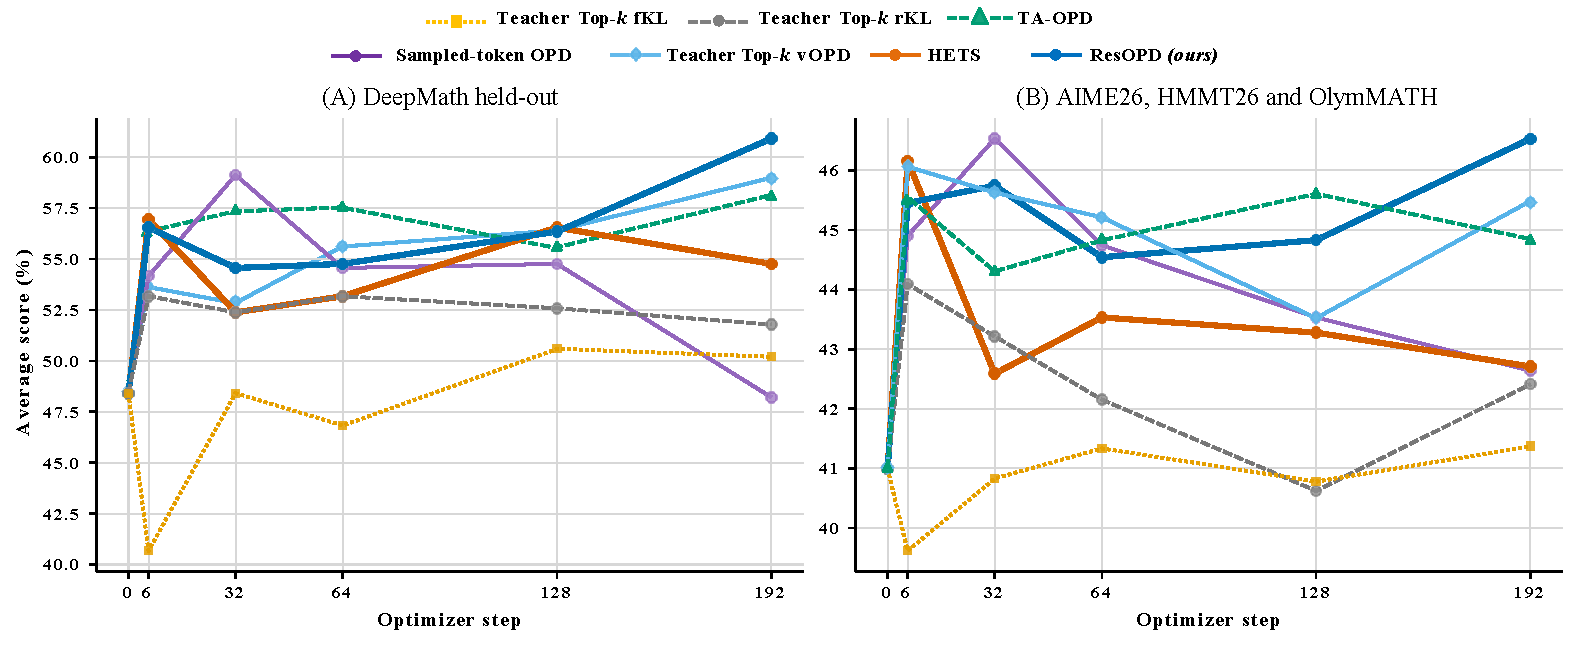
\includegraphics[width=0.85\textwidth]{figs/math_step_v4.pdf}
\caption{\textbf{Step-wise learning curves} corresponding to Tab.~\ref{tab:math-terminal} on DeepMath held-out (left) and external competitions (right) across 192 optimizer steps.}
\label{fig:estimator-learning}
\end{figure}

Fig.~\ref{fig:qwen3-transfer-curves} illustrates the checkpoint evaluation trajectories along the fixed training progression (steps 0, 10, 25, 50, and 100) across all four benchmarks. On code benchmarks (LiveCodeBench v5 and v6), ResOPD and HETS rapidly converge and consistently outperform Sampled-token OPD by a substantial margin throughout training, with ResOPD achieving the highest overall trajectory AUC. In contrast, science benchmarks display mixed domain dynamics: Sampled-token OPD demonstrates superior retention and final accuracy on GPQA-D, whereas ResOPD remains competitive across training steps and achieves the best terminal performance on SuperGPQA. These trajectories corroborate that while Sampled-token OPD remains strong in specialized scientific reasoning, ResOPD provides transfer performance on code tasks without sacrificing overall multi-domain balance.

\begin{figure}[htbp]
  \centering
  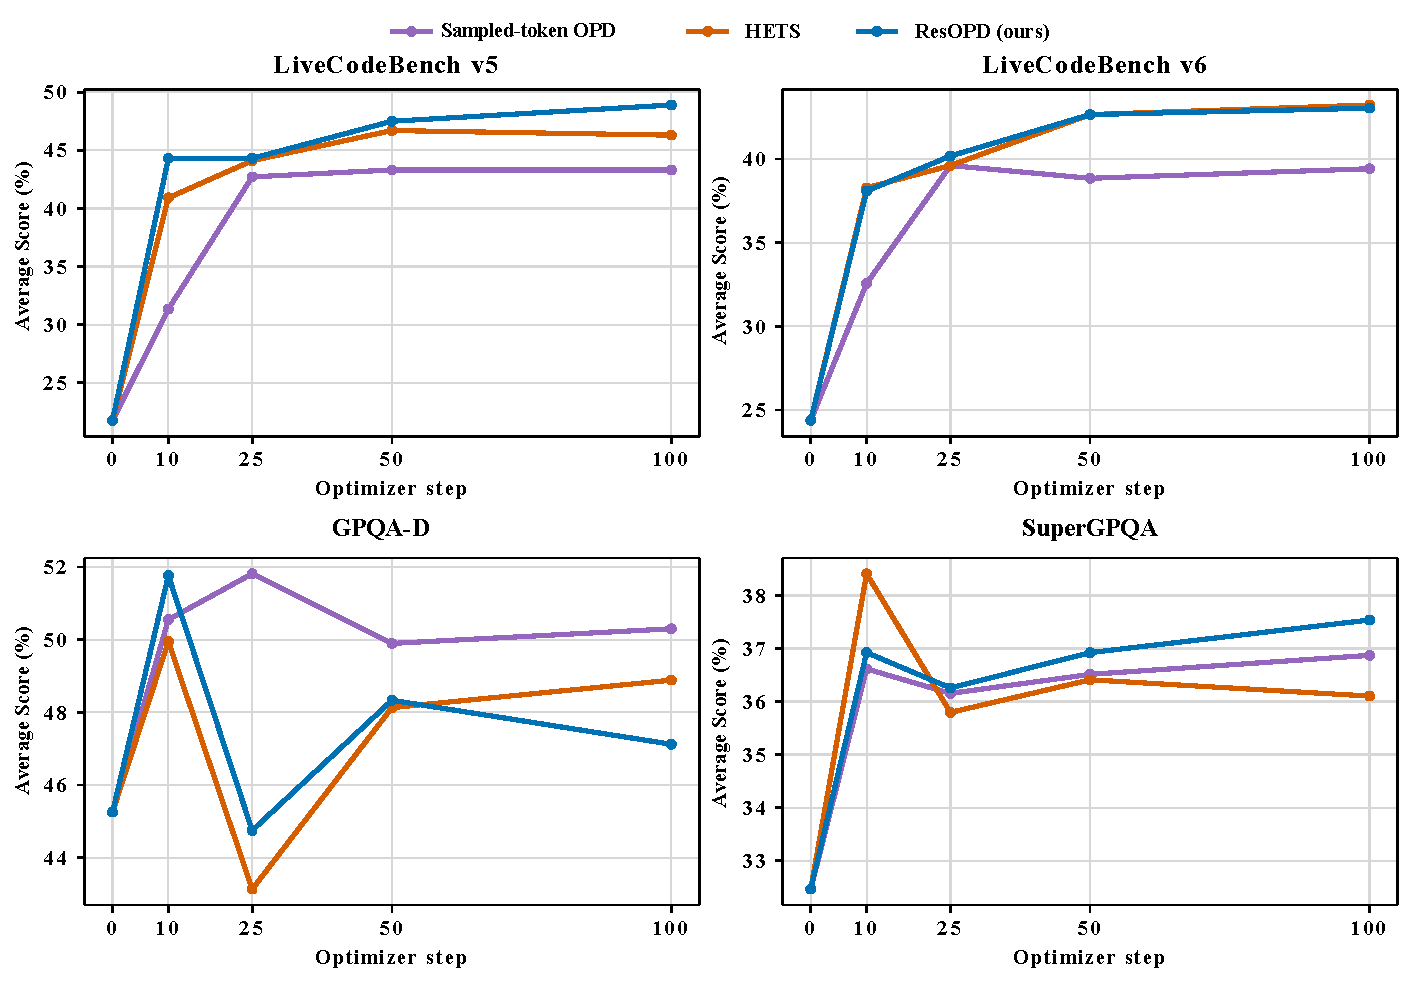
\includegraphics[width=0.85\columnwidth]{figs/qwen3_4b30_transfer_curves_v2.pdf}
    \caption{\textbf{Evaluation trajectories during cross-domain transfer distillation} from Qwen3-30B-A3B-Instruct to Qwen3-4B across optimizer steps (0, 10, 25, 50, and 100).}
    \label{fig:qwen3-transfer-curves}
\end{figure}

\FloatBarrier
\section{Details of diagnostics}
\label{app:math-curves}

\subsection{What the online residual moments measure}
\label{app:online-residual-moments}

At optimizer update $u$, let $i \in \{1, \dots, B_u\}$ index the non-empty sampled responses and $t \in \{1, \dots, T_{ui}\}$ index their valid tokens. We define the scalar support residual and its components as
\begin{equation}
  P_{uit} \coloneqq p_\theta(S_{uit} \mid x_{uit}), \qquad
  H_{uit} \coloneqq \ind\{A_{uit} \in S_{uit}\}, \qquad
  Z_{uit} \coloneqq H_{uit} - P_{uit}.
  \label{eq:online-support-residual}
\end{equation}
Here, $P_{uit}$ denotes the Student probability mass allocated to the transmitted Teacher \text{Top-}$k$ support $S_{uit}$, while $H_{uit}$ indicates whether the sampled Student token lands within this set. Under an exact on-policy draw, the residual is conditionally zero-mean, $\E[Z_{uit} \mid x_{uit}] = 0$, with conditional variance $\E[Z_{uit}^2 \mid x_{uit}] = P_{uit}(1 - P_{uit})$. More generally, its uncentered second moment captures both intrinsic sampling variability and any realized calibration drift.

Fig.~\ref{fig:training-dynamics-event-g0} reports two diagnostic aggregations of this quantity. Panel~C displays the masked token-level second moment:
\begin{equation}
  M_{2,\mathrm{tok}}^{(u)} = \frac{1}{\sum_{i=1}^{B_u} T_{ui}} \sum_{i=1}^{B_u} \sum_{t=1}^{T_{ui}} Z_{uit}^2,
  \label{eq:online-token-m2}
\end{equation}
whereas Panel~D evaluates the trajectory-level variance by first averaging within each response and then weighting responses uniformly:
\begin{equation}
  \bar{Z}_{ui} = \frac{1}{T_{ui}} \sum_{t=1}^{T_{ui}} Z_{uit}, \qquad
  M_{2,\mathrm{traj}}^{(u)} = \frac{1}{B_u} \sum_{i=1}^{B_u} \bar{Z}_{ui}^2.
  \label{eq:online-trajectory-m2}
\end{equation}
Intuitively, $M_{2,\mathrm{tok}}$ captures the instantaneous magnitude of the unresolved head-versus-tail events (which is leveraged in Fig.~\ref{fig:topk-ablation} to approximate the between-event variance factor $P\tau_p$), whereas $M_{2,\mathrm{traj}}$ measures the persistent, signed event imbalance surviving along sequence rollouts. Defining the batch mean $\bar{Z}_u = B_u^{-1} \sum_{i=1}^{B_u} \bar{Z}_{ui}$, the empirical standard error of the trajectory mean is given by
\begin{equation}
  \widehat{\operatorname{SE}}(\bar{Z}_u) = \sqrt{\frac{\max\{M_{2,\mathrm{traj}}^{(u)} - \bar{Z}_u^2, 0\}}{B_u - 1}}.
  \label{eq:online-trajectory-se}
\end{equation}

The connection to ResOPD is exact at the scalar-coefficient level. Noting that tail indicators and tail masses satisfy $J_{uit} = 1 - H_{uit}$ and $\tau_{p,uit} = 1 - P_{uit}$, we obtain $Z_{uit} = \tau_{p,uit} - J_{uit}$. Substituting this into Equation~(\ref{eq:residualization}) yields
\begin{equation}
  \widehat{\bgrad}_{uit}^{\mathrm{ResOPD}} - \widehat{\bgrad}_{uit}^{\mathrm{HETS}} = Z_{uit} \bmean_{B,uit}.
  \label{eq:online-residual-cfr-link}
\end{equation}
Hence, the two $M_2$ metrics directly track the magnitude and sequence-level persistence of the random scalar modulating ResOPD's bucket control. Because they intentionally abstract away $\lVert\bmean_{B,uit}\rVert$, its alignment with the fine-tail mean, and the orthogonal within-tail fluctuations, they serve as computationally lightweight, mechanism-aligned online diagnostics rather than full covariance estimators or replacements for fixed-prefix NSR. Finally, while $Z$ can trivially be recorded for a sparse Top-$k$ objective, direct Top-$k$ rKL lacks a sampled tail correction and remains inherently biased with respect to the true rKL target. Its zero action-sampling variance is therefore not comparable to the unbiased vOPD, HETS and ResOPD estimators in Panels~C and~D.

% UNIFIED_DIAGNOSTICS_END

\subsection{Finite gradient-enumeration check}
\label{app:finite-check}

We also verify the unbiasedness identities without Monte Carlo error on a
four-action softmax. The Student and Teacher probabilities are respectively
$(0.35,0.30,0.20,0.15)$ and $(0.60,0.25,0.10,0.05)$, and the first two actions form the
Teacher Top-2 support. We differentiate the full reverse KL directly, enumerate
each possible Student action, and weight its estimator gradient by the exact
Student action probability. The resulting HETS expectation matches the dense
full-rKL gradient to maximum absolute error $5.6\times10^{-17}$.

ResOPD changes the per-action vector by
$(\tau_p-J)\bmean_B$ relative to HETS. Because the same enumeration has
$\E[J]=\tau_p$, this correction sums exactly to zero and ResOPD recovers the same
dense gradient. This finite check complements the symbolic identity in
Equation~(\ref{eq:residualization}): it validates the stopped-coefficient and
support-mask implementation semantics, but it is not empirical evidence about
covariance or downstream accuracy.

\subsection{Complete frozen-prefix support diagnostics}
\label{app:fixed-prefix-sweep}

\begin{table}[t]
\caption{\textbf{Support-size ($k$) sweep under fixed Teacher Top-$k$ payloads.}
``Var.~Removed'' measures the empirical covariance-trace reduction relative to sampled-token OPD. Payload accounts for $k$ Top-$k$ entries plus the sampled token (INT32 ID and FP32 log-probability each). Student mass and Head Hit denote the predicted and empirical probabilities of landing in the Top-$k$ support, respectively. Best variance reduction and NSR per setting are in \textbf{bold}.}
\label{tab:fixed-prefix-sweep}
\centering
\small
\renewcommand{\arraystretch}{1.16}
\setlength{\tabcolsep}{4.0pt}

\begin{tabular*}{\textwidth}{@{\extracolsep{\fill}}lrrccrrrr@{}}
\toprule
\multirow{2}{*}{\shortstack[l]{Dataset \\ Student/Teacher}}
& \multirow{2}{*}{$k$}
& \multirow{2}{*}{\shortstack{Payload \\ (B/token)}}
& \multirow{2}{*}{\shortstack{Student \\ mass}}
& \multirow{2}{*}{\shortstack{Head \\ Hit}}
& \multicolumn{2}{c}{Var. Removed (\%) $\uparrow$}
& \multicolumn{2}{c}{NSR $\downarrow$} \\
\cmidrule(lr){6-7}\cmidrule(l){8-9}
& & & & & HETS & ResOPD & HETS & ResOPD \\
\midrule
\multirow{4}{*}{\shortstack[l]{\textbf{GSM8K} \\ 0.8B/4B}}
& 1  & 16  & $75.0\%$ & $74.8\%$  & $-0.5$ & $\mathbf{20.5}$ & 5.446 & $\mathbf{4.310}$ \\
& 4  & 40  & $93.1\%$ & $92.9\%$  & 27.3   & $\mathbf{52.5}$ & 3.940 & $\mathbf{2.573}$ \\
& 16 & 136 & $97.7\%$ & $97.9\%$  & 62.6   & $\mathbf{75.3}$ & 2.027 & $\mathbf{1.337}$ \\
& 64 & 520 & $99.3\%$ & $99.7\%$  & 85.1   & $\mathbf{89.5}$ & 0.807 & $\mathbf{0.570}$ \\
\addlinespace[0.25em]
\multirow{3}{*}{\shortstack[l]{\textbf{HMMT26} \\ 4B/27B}}
& 1  & 16  & $89.1\%$ & $89.3\%$   & $-1.0$ & $\mathbf{32.0}$ & 6.656 & $\mathbf{4.479}$ \\
& 4  & 40  & $99.1\%$ & $98.8\%$   & 55.8   & $\mathbf{75.3}$ & 2.914 & $\mathbf{1.630}$ \\
& 16 & 136 & $99.9\%$ & $100.0\%$  & 89.8   & $\mathbf{94.2}$ & 0.675 & $\mathbf{0.382}$ \\
\bottomrule
\end{tabular*}
\end{table}


\begin{figure}[t]
\centering
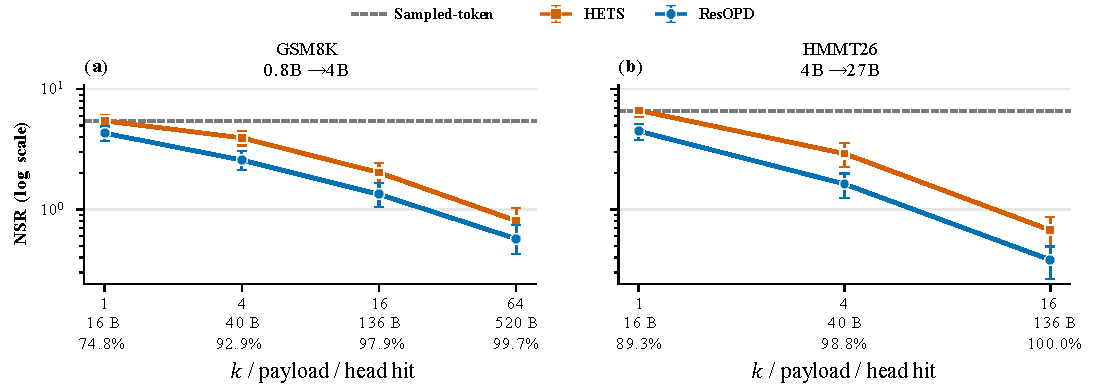
\includegraphics[width=0.96\textwidth]{figs/fixed_prefix_support_strata_v2.pdf}
\caption{\textbf{Comprehensive frozen-prefix support-size ($k$) diagnostics across benchmarks.} 
ResOPD consistently reduces the dimensionless NSR across all evaluated support sizes on GSM8K and HMMT (log scale). Axis annotations detail the transmitted Teacher support size $k$, the corresponding communication payload (bytes/token), and the empirical head-hit probability. Error bars denote 95\% trajectory-level bootstrap confidence intervals.}
\label{fig:fixed-prefix-diagnostics}
\end{figure}

Across both suites in Tab.~\ref{tab:fixed-prefix-sweep}, ResOPD consistently outperforms HETS at every matched support size, achieving higher covariance-trace elimination and lower NSR. Expanding $k$ from $4$ to $16$ and $64$ scales transmission costs by $3.4\times$ and $13\times$ ($40 \to 136 \to 520$\,B/token) for diminishing marginal variance gains. Crucially, the head hit rates demonstrate why high support coverage alone is insufficient: even when head mass reaches $98.8\%$ ($k=4$ on HMMT26), the rare $1.2\%$ tail draws still induce a substantial HETS--ResOPD variance gap ($55.8\%$ vs.\ $75.3\%$ removed). Moreover, at $k=1$ where HETS exhibits negative reduction ($-1.0\%$), ResOPD reliably eliminates $32.0\%$ of the gradient variance. This firmly corroborates the theoretical condition in Equation~(\ref{eq:hets-cfr-variance-appendix}), confirming that uncorrected tail draws dominate residual gradient noise despite their low nominal probability mass.

\subsection{Training dynamics across learning rates}
\label{app:lr-sensitivity}


\paragraph{Underlying training dynamics.}
The training trajectories in Fig.~\ref{fig:lr-sensitivity} reveal two clear mechanisms behind this divergence. First, in terms of gradient magnitude, ResOPD maintains substantially lower pre-clipping gradient norms at $5\times10^{-6}$ (mean $0.43$ vs.\ $0.48$; p99 $0.97$ vs.\ $1.84$) and completely avoids gradient clipping ($0/64$ steps vs.\ $2/64$ steps for HETS). Second, regarding residual stabilization, Panels~(B)--(D) show that ResOPD consistently curbs the support-mass gap ($Q-P$) and suppresses both token- and trajectory-level residual second moments ($M_2$), consistent with the more stable learning trajectory observed at this step size.

\begin{figure}[t]
  \centering
  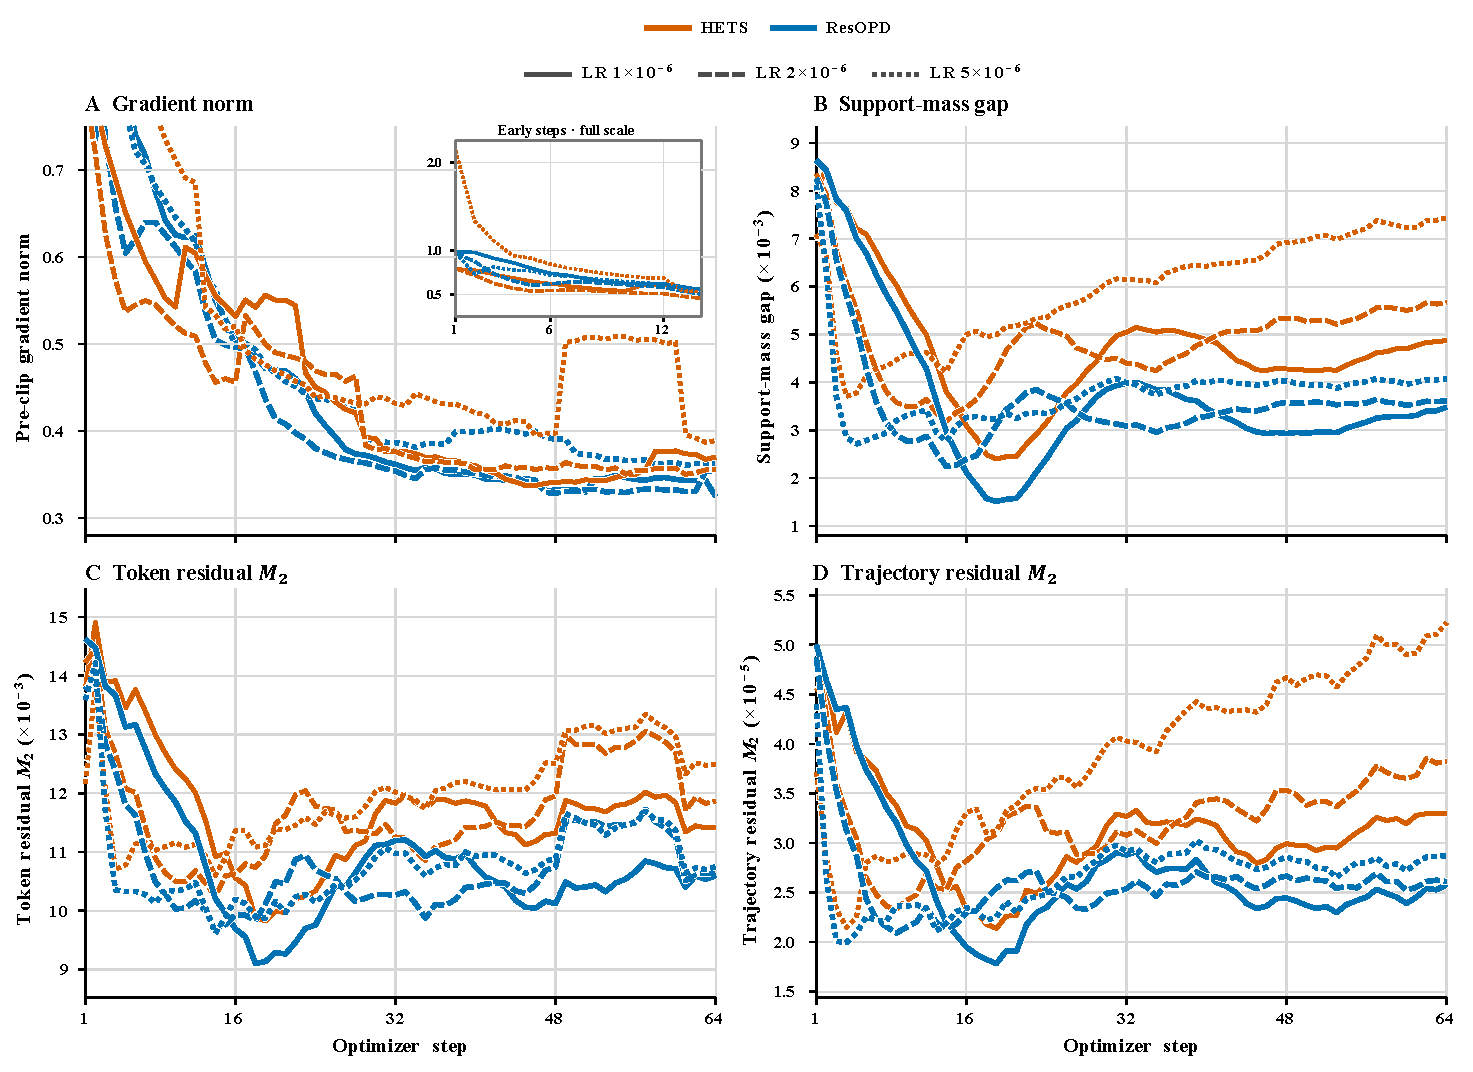
\includegraphics[width=0.9\columnwidth]{figs/lr_training_dynamics_cfr_v3.pdf}
  \caption{\textbf{Training dynamics and learning-rate sensitivity} of HETS (\textit{orange}) vs.\ ResOPD (\textit{blue}) on DeepMath across three learning rates ($1\times10^{-6}$ solid, $2\times10^{-6}$ dashed, $5\times10^{-6}$ dotted).
  \textbf{(A)} Pre-clipping global gradient norm (inset displays full-scale unclipped peaks over early steps).
  \textbf{(B)} Support-mass gap ($Q - P$) on the transmitted Teacher Top-4 tokens.
  \textbf{(C, D)} Token-level and trajectory-level second residual moments ($M_2$).
  While HETS exhibits large gradient-norm excursions and growing mass/residual discrepancies as the learning rate scales up to $5\times10^{-6}$, ResOPD maintains stable dynamics and stays close to its low-rate trajectories throughout optimization.}
  \label{fig:lr-sensitivity}
\end{figure}